% Buy or Wait? -- Architecture and Design Document
% Build: latexmk -pdf architecture.tex   (or: tectonic architecture.tex)
\documentclass[11pt,a4paper]{article}

\usepackage[margin=2.2cm]{geometry}
\usepackage[T1]{fontenc}
\usepackage{lmodern}
\usepackage{microtype}
\usepackage{amsmath,amssymb}
\usepackage{booktabs,longtable,array,tabularx}
\usepackage{xcolor}
\usepackage{enumitem}
\usepackage{tikz}
\usetikzlibrary{arrows.meta,positioning,fit,backgrounds,calc,shapes.geometric,shapes.multipart}
\usepackage{pgfplots}
\pgfplotsset{compat=1.17}
\usepackage[hidelinks]{hyperref}
\usepackage{listings}

\definecolor{ink}{HTML}{1F2937}
\definecolor{accent}{HTML}{2563EB}
\definecolor{ok}{HTML}{15803D}
\definecolor{warn}{HTML}{B45309}
\definecolor{bad}{HTML}{B91C1C}
\definecolor{soft}{HTML}{EEF2FF}
\definecolor{softg}{HTML}{ECFDF5}
\definecolor{softy}{HTML}{FFFBEB}
\definecolor{softr}{HTML}{FEF2F2}
\definecolor{grey}{HTML}{6B7280}

\lstset{basicstyle=\ttfamily\small,columns=fullflexible,breaklines=true,frame=single,rulecolor=\color{grey}}

\tikzset{
  box/.style={draw=ink,rounded corners=3pt,fill=white,align=center,font=\small,inner sep=5pt,minimum height=9mm},
  store/.style={draw=ink,cylinder,shape border rotate=90,aspect=0.18,fill=softy,align=center,font=\small,minimum height=12mm,minimum width=22mm},
  ext/.style={draw=grey,dashed,rounded corners=3pt,fill=soft,align=center,font=\small,inner sep=5pt,minimum height=9mm},
  model/.style={draw=accent,thick,rounded corners=3pt,fill=soft,align=center,font=\small,inner sep=5pt,minimum height=9mm},
  good/.style={draw=ok,thick,rounded corners=3pt,fill=softg,align=center,font=\small,inner sep=5pt},
  fail/.style={draw=bad,thick,rounded corners=3pt,fill=softr,align=center,font=\small,inner sep=5pt},
  decision/.style={draw=ink,diamond,aspect=2.2,fill=softy,align=center,font=\footnotesize,inner sep=1pt},
  flow/.style={-{Stealth[length=2.2mm]},thick,draw=ink},
  dflow/.style={-{Stealth[length=2.2mm]},thick,dashed,draw=grey},
  lbl/.style={font=\footnotesize,fill=white,inner sep=1pt},
  group/.style={draw=grey,rounded corners=6pt,inner sep=8pt,fill=gray!4},
  grouplabel/.style={font=\footnotesize\bfseries,text=grey,anchor=north west}
}

\title{\textbf{Buy or Wait?}\\[2pt]\large Architecture and Design of a Verified-or-Fail-Closed Financial Decision Agent}
\author{HackerRank Orchestrate --- September 2026}
\date{Revision: main \texttt{fbe1c4a} (verifier sign-off on \texttt{3c77c81})}

\begin{document}
\maketitle

\begin{abstract}
\noindent Buy or Wait? decides, for every purchase or payment request, how much is safe to pay today, whether
the user can afford it now, with a plan, later, or not at all, and which payment method, schedule and
spending changes to recommend. The system is a single Rust crate. A deterministic decision engine
reconstructs each user's cash position from structured financial events, fixed dated exchange rates,
supplied payment options and evidence from messages and receipt images, then forecasts the balance
day by day against the user's minimum balance. Receipt images are read at ingestion by a self-hosted
OCR model (\texttt{baidu/Unlimited-OCR} on vLLM) and cached. Every figure the engine uses from an image
is mapped deterministically from printed labels and must pass a witness gate, or it fails closed and is
never guessed. The final run produced 250 decisions, 0 contract violations, 0 wrong image figures
and byte-identical output across two cold runs.
\end{abstract}

\tableofcontents
\newpage

%=====================================================================
\section{Goals and design principles}
%=====================================================================

\begin{enumerate}[leftmargin=*,itemsep=2pt]
  \item \textbf{Contract-exact output.} One row per \texttt{request\_id} in \texttt{dataset/requests.csv}, with the
        exact 8-column header, enumerations and field semantics of \texttt{AGENTS.md}~\S6.2.
  \item \textbf{Verified or fail closed.} No figure enters the ledger unless it is proven. An unproven image or message
        figure is dropped with a recorded reason, never estimated. Wrong figures must be 0.
  \item \textbf{Determinism.} Two \texttt{--cold} runs produce byte-identical \texttt{output.csv}. Money is fixed-point,
        models run at temperature 0, and every model output is cached with a config hash.
  \item \textbf{Models read, Rust decides.} Models only transcribe. Every financial interpretation (which figure,
        cash treatment, plan ranking, explanation) is deterministic Rust.
  \item \textbf{Conservative safety.} The balance never falls below \texttt{minimum\_balance\_to\_keep} after any projected
        essential expense or recommended payment. Pending debits are reserved; unsettled credits are not counted.
  \item \textbf{Operable and auditable.} Terminal-runnable, secrets from environment only, a per-request
        \texttt{DecisionFacts} record, persisted provenance for every image read, and a usage report for the final run.
\end{enumerate}

%=====================================================================
\section{System context}
%=====================================================================

The product shape is a two-phase system. Users upload receipts and documents first; ingestion OCRs them once
and caches the result. Questions (\emph{``can I afford this?''}) are then answered from the cached, verified evidence.
The submission runs both phases in batch over the dataset.

\begin{figure}[h]
\centering
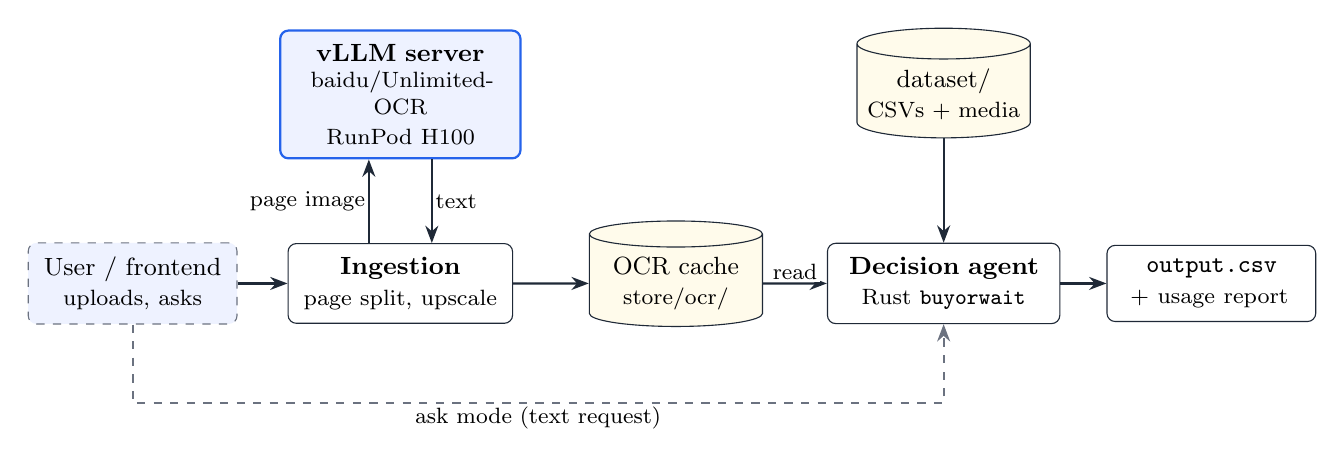
\begin{tikzpicture}[font=\small]
  \node[ext, text width=2.3cm] (user) at (0,0) {User / frontend\\\footnotesize uploads, asks};
  \node[box, text width=2.5cm] (ingest) at (3.4,0) {\textbf{Ingestion}\\\footnotesize page split, upscale};
  \node[model, text width=2.7cm] (vllm) at (3.4,2.4) {\textbf{vLLM server}\\\footnotesize baidu/Unlimited-OCR\\\footnotesize RunPod H100};
  \node[store] (cache) at (6.9,0) {OCR cache\\\footnotesize store/ocr/};
  \node[box, text width=2.6cm] (agent) at (10.3,0) {\textbf{Decision agent}\\\footnotesize Rust \texttt{buyorwait}};
  \node[store] (data) at (10.3,2.4) {dataset/\\\footnotesize CSVs + media};
  \node[box, text width=2.3cm] (out) at (13.7,0) {\texttt{output.csv}\\\footnotesize + usage report};
  \draw[flow] (user) -- (ingest);
  \draw[flow] ([xshift=-4mm]ingest.north) -- node[lbl,left]{page image} ([xshift=-4mm]vllm.south);
  \draw[flow] ([xshift=4mm]vllm.south) -- node[lbl,right]{text} ([xshift=4mm]ingest.north);
  \draw[flow] (ingest) -- (cache);
  \draw[flow] (cache) -- node[lbl,above]{read} (agent);
  \draw[flow] (data) -- (agent);
  \draw[flow] (agent) -- (out);
  \draw[dflow] (user.south) -- ++(0,-1.0) -| node[lbl,pos=0.25,below]{ask mode (text request)} (agent.south);
\end{tikzpicture}
\caption{Context. The OCR model sits behind an OpenAI-compatible vLLM endpoint and is called only at ingestion. The decision agent reads the cache.}
\end{figure}

%=====================================================================
\section{Crate structure}
%=====================================================================

\begin{figure}[h]
\centering
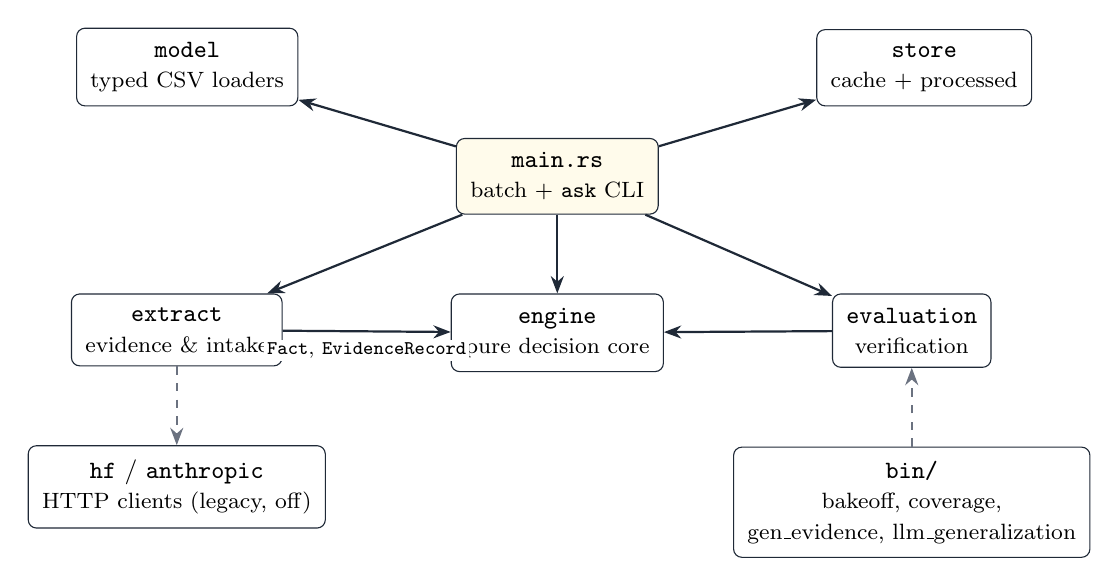
\begin{tikzpicture}[node distance=6mm and 8mm]
  \node[box,fill=softy] (main) {\texttt{main.rs}\\\footnotesize batch + \texttt{ask} CLI};
  \node[box, below left=10mm and 22mm of main] (extract) {\texttt{extract}\\\footnotesize evidence \& intake};
  \node[box, below=10mm of main] (engine) {\texttt{engine}\\\footnotesize pure decision core};
  \node[box, below right=10mm and 22mm of main] (eval) {\texttt{evaluation}\\\footnotesize verification};
  \node[box, above left=4mm and 20mm of main] (model) {\texttt{model}\\\footnotesize typed CSV loaders};
  \node[box, above right=4mm and 20mm of main] (store) {\texttt{store}\\\footnotesize cache + processed};
  \node[box, below=10mm of extract] (hf) {\texttt{hf} / \texttt{anthropic}\\\footnotesize HTTP clients (legacy, off)};
  \node[box, below=10mm of eval] (bins) {\texttt{bin/}\\\footnotesize bakeoff, coverage,\\\footnotesize gen\_evidence, llm\_generalization};
  \draw[flow] (main) -- (extract); \draw[flow] (main) -- (engine); \draw[flow] (main) -- (eval);
  \draw[flow] (main) -- (model);   \draw[flow] (main) -- (store);
  \draw[flow] (extract) -- node[lbl,below=1mm,font=\scriptsize]{\texttt{Fact}, \texttt{EvidenceRecord}} (engine);
  \draw[flow] (eval) -- (engine);
  \draw[dflow] (extract) -- (hf);
  \draw[dflow] (bins) -- (eval);
\end{tikzpicture}
\caption{Module dependencies. \texttt{engine} has no I/O, network or model calls. \texttt{extract} converts evidence into the engine's own \texttt{Fact} contract and never decides cash treatment.}
\end{figure}

\begin{longtable}{>{\ttfamily}p{3.6cm} p{11.6cm}}
\toprule
\normalfont\textbf{Module} & \textbf{Responsibility}\\\midrule
\endhead
engine::money & Fixed-point money in $10^{-4}$ currency units; rounding only at output.\\
engine::rules & All tunable decision rules and toggles (\texttt{Rules::default()}).\\
engine::session & One user: profile, events, rates; entry point \texttt{Session::from\_model}.\\
engine::ledger & Cash rules by status and direction, lifecycle de-duplication, evidence amendments in the spec's conflict order, FX conversion, \texttt{Fact} application.\\
engine::recurrence & Detects recurring streams (salary, bills, variable spend) only where history supports them.\\
engine::forecast & Day-by-day balance projection, safe amount and earliest full-payment date.\\
engine::plans & Candidate plans (full, installments, two-payment partial, wait, spending changes), eligibility, safety replay, ranking.\\
engine::facts & \texttt{DecisionFacts}: every number the decision rests on.\\
engine::explain & Template explanations rendered only from \texttt{DecisionFacts} (0 tokens).\\
extract::messages & Typed message records and a deterministic parser for known message families.\\
extract::grounding & A number claimed from a message must literally appear in its text.\\
extract::retrieval & Per-user, date-bounded message evidence retrieval.\\
extract::ocr & vLLM client, page splitting, conditional upscaling, config-hashed cache, usage.\\
extract::ocr\_parse & Raw OCR (HTML tables, \texttt{<|det|>} blocks) into label:value rows, including zipping multi-value cells.\\
extract::labels & Deterministic keyword to role mapping into \texttt{ImageFigures}.\\
extract::normalize & Trap-aware amount, currency and date parsing (lakh grouping, comma decimals, Rs/Ps splits).\\
extract::witness & Witness identities, amount-in-words parser, contradiction checks.\\
extract::images & Selector by event type and status, witness gate, provenance (\texttt{ImageReadProvenance}).\\
extract::intake & \texttt{ask}-mode free-text request intake (not used in batch).\\
store::cache / processed & Model-call cache and persisted preprocessing (ledgers, image reads).\\
evaluation::* & Contract validator, invariants, sample scorer, replay mirror, false-accept gate, image agreement, hardcode scan, sign-off.\\
\bottomrule
\end{longtable}

%=====================================================================
\section{Batch pipeline}
%=====================================================================

\begin{figure}[h]
\centering
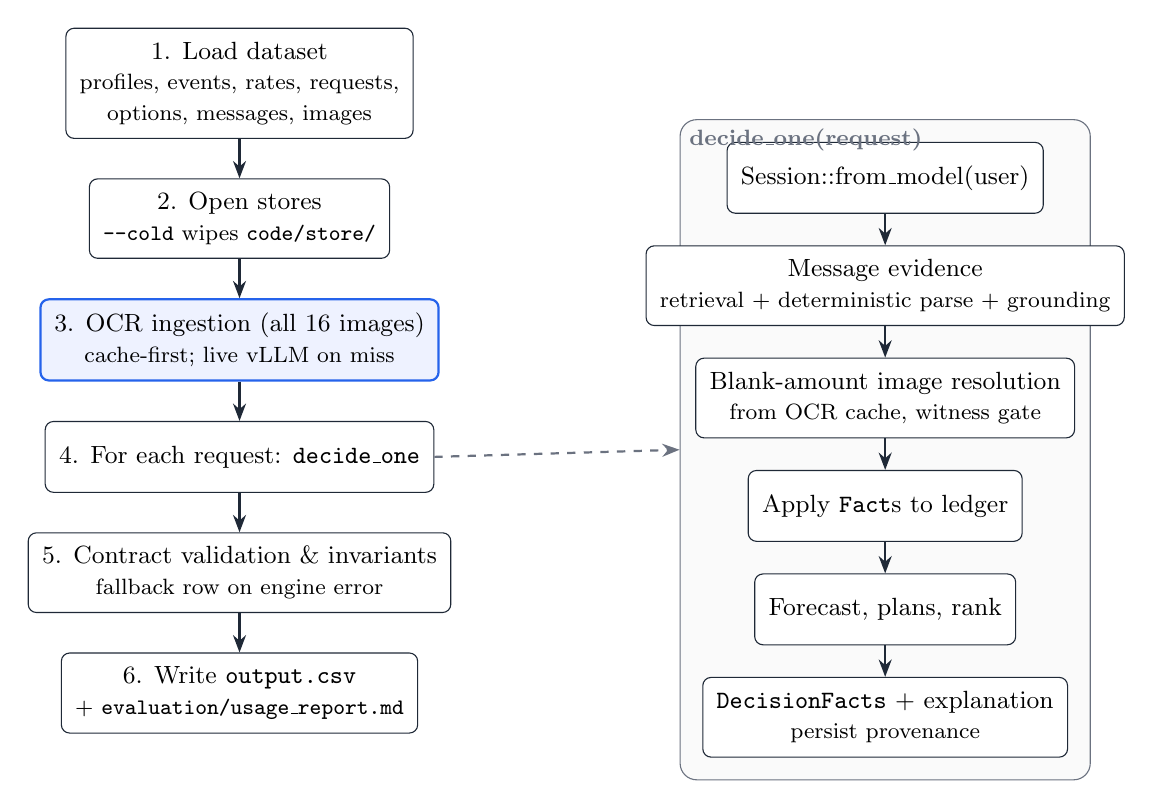
\begin{tikzpicture}[node distance=5mm]
  \node[box] (s1) {1. Load dataset\\\footnotesize profiles, events, rates, requests,\\\footnotesize options, messages, images};
  \node[box, below=of s1] (s2) {2. Open stores\\\footnotesize \texttt{--cold} wipes \texttt{code/store/}};
  \node[model, below=of s2] (s3) {3. OCR ingestion (all 16 images)\\\footnotesize cache-first; live vLLM on miss};
  \node[box, below=of s3] (s4) {4. For each request: \texttt{decide\_one}};
  \node[box, below=of s4] (s5) {5. Contract validation \& invariants\\\footnotesize fallback row on engine error};
  \node[box, below=of s5] (s6) {6. Write \texttt{output.csv}\\\footnotesize + \texttt{evaluation/usage\_report.md}};
  \foreach \a/\b in {s1/s2,s2/s3,s3/s4,s4/s5,s5/s6} \draw[flow] (\a) -- (\b);

  \begin{scope}[xshift=8.2cm,yshift=-1.2cm,node distance=4mm]
    \node[box] (d1) {Session::from\_model(user)};
    \node[box, below=of d1] (d2) {Message evidence\\\footnotesize retrieval + deterministic parse + grounding};
    \node[box, below=of d2] (d3) {Blank-amount image resolution\\\footnotesize from OCR cache, witness gate};
    \node[box, below=of d3] (d4) {Apply \texttt{Fact}s to ledger};
    \node[box, below=of d4] (d5) {Forecast, plans, rank};
    \node[box, below=of d5] (d6) {\texttt{DecisionFacts} + explanation\\\footnotesize persist provenance};
    \foreach \a/\b in {d1/d2,d2/d3,d3/d4,d4/d5,d5/d6} \draw[flow] (\a) -- (\b);
    \begin{scope}[on background layer]
      \node[group, fit=(d1)(d6)] (g) {};
    \end{scope}
    \node[grouplabel] at (g.north west) {decide\_one(request)};
  \end{scope}
  \draw[dflow] (s4.east) -- (g.west);
\end{tikzpicture}
\caption{Batch control flow (\texttt{code/src/main.rs}). Requests are independent; per-user state is rebuilt for each request.}
\end{figure}

%=====================================================================
\section{Image evidence pipeline}
%=====================================================================

Sixteen financial events have blank amounts whose values are printed on images (receipts, bills, a payslip, a
handwritten pharmacy bill). Four of them are pending or scheduled and therefore change a forecast.

\subsection{Why OCR plus deterministic mapping}
An audit of earlier vision-language-model reads (Qwen3-VL-235B, gemma-4-31B) found that the models transcribed every
printed final amount correctly. Every failure came from asking the model to \emph{interpret} the page into fixed JSON keys:
it invented totals, subtotals, balances and due-date cutoffs the page did not print. The redesign lets the model only
transcribe what is printed; Rust assigns meaning from the printed label text.

\begin{figure}[h]
\centering
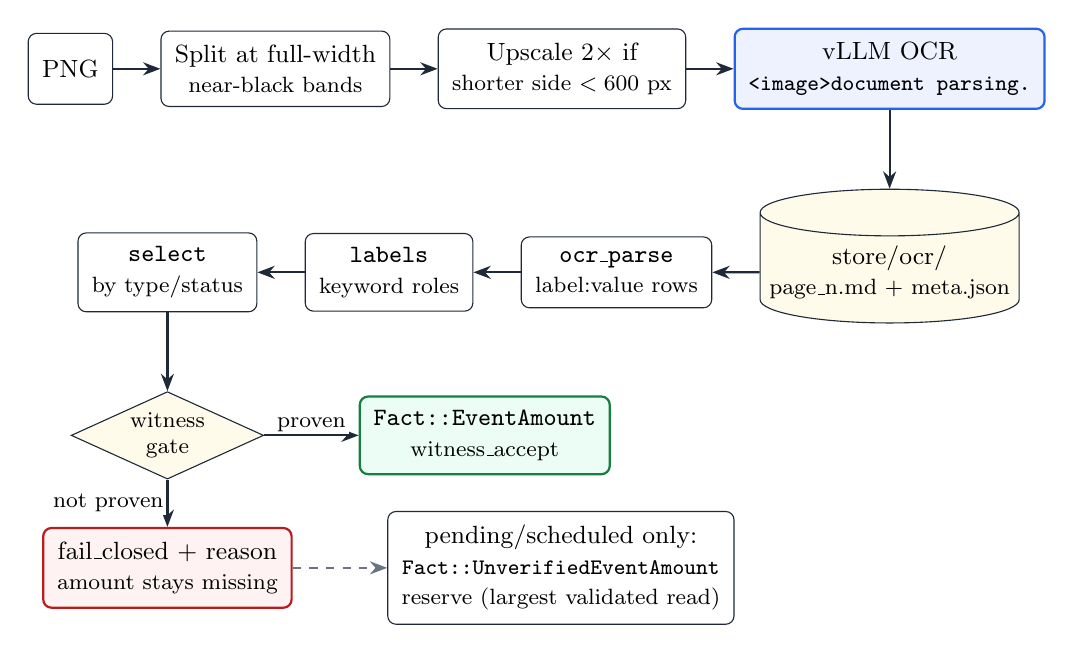
\begin{tikzpicture}[node distance=5mm and 6mm]
  \node[box] (png) {PNG};
  \node[box, right=of png] (split) {Split at full-width\\\footnotesize near-black bands};
  \node[box, right=of split] (up) {Upscale $2\times$ if\\\footnotesize shorter side $<600$ px};
  \node[model, right=of up] (ocr) {vLLM OCR\\\footnotesize \texttt{<image>document parsing.}};
  \node[store, below=10mm of ocr] (c) {store/ocr/\\\footnotesize page\_n.md + meta.json};
  \node[box, left=of c] (parse) {\texttt{ocr\_parse}\\\footnotesize label:value rows};
  \node[box, left=of parse] (labels) {\texttt{labels}\\\footnotesize keyword roles};
  \node[box, left=of labels] (sel) {\texttt{select}\\\footnotesize by type/status};
  \node[decision, below=10mm of sel] (gate) {witness\\gate};
  \node[good, right=12mm of gate] (acc) {\texttt{Fact::EventAmount}\\\footnotesize witness\_accept};
  \node[fail, below=6mm of gate] (fc) {fail\_closed + reason\\\footnotesize amount stays missing};
  \node[box, right=12mm of fc] (res) {pending/scheduled only:\\\footnotesize \texttt{Fact::UnverifiedEventAmount}\\\footnotesize reserve (largest validated read)};
  \draw[flow] (png) -- (split); \draw[flow] (split) -- (up); \draw[flow] (up) -- (ocr);
  \draw[flow] (ocr) -- (c); \draw[flow] (c) -- (parse); \draw[flow] (parse) -- (labels); \draw[flow] (labels) -- (sel);
  \draw[flow] (sel) -- (gate); \draw[flow] (gate) -- node[lbl,above]{proven} (acc);
  \draw[flow] (gate) -- node[lbl,left]{not proven} (fc); \draw[dflow] (fc) -- (res);
\end{tikzpicture}
\caption{Image pipeline. OCR runs once per page at ingestion; everything after the cache is deterministic.}
\end{figure}

\subsection{OCR serving configuration}
\begin{tabularx}{\textwidth}{>{\bfseries}p{4cm} X}
\toprule
Model & \texttt{baidu/Unlimited-OCR} (MIT, 3.34B parameters, BF16; DeepSeek-OCR lineage)\\
Server & \texttt{vllm/vllm-openai:unlimited-ocr-cu129}, \texttt{--trust-remote-code}, \texttt{--logits\_processors ...NGramPerReqLogitsProcessor}, prefix and multimodal caches disabled\\
Request & one image per request; \texttt{temperature=0}, \texttt{max\_tokens=8192}, \texttt{skip\_special\_tokens=false}, \texttt{vllm\_xargs=\{ngram\_size:35, window\_size:128\}}; explicit User-Agent (the RunPod proxy rejects requests without one)\\
Environment & \texttt{OCR\_BASE\_URL}, \texttt{OCR\_MODEL}, optional \texttt{OCR\_API\_KEY}\\
Cache key & config hash over model, prompt, token limit, n-gram arguments, page scale and split thresholds\\
Final cold run & 17 pages (16 images; one stitched two-page invoice), 31{,}309 prompt + 11{,}703 completion = 43{,}012 tokens, 53.6\,s wall time; two runs byte-identical over all 16 images\\
\bottomrule
\end{tabularx}

\subsection{Label to role mapping}
\texttt{extract::labels} maps each printed label with a fixed keyword list. No model decides meaning.
\begin{center}\small
\begin{tabularx}{\textwidth}{@{}>{\ttfamily}p{4.2cm}X@{}}
\toprule
\normalfont Role & Printed-label keywords (examples)\\\midrule
grand\_total & Grand Total\\
total & Total, Total Amount, Total Bill Amount, Net Amount, Total paid, Total Amount Received\\
amount\_paid & Amount Received, Amount Paid, Total paid\\
balance\_due / amount\_due & Balance Due, Balance / Amount Payable, Amount Due\\
subtotal & Sub Total, Item Bill, Item Total, Taxable Value (never promoted to total)\\
tax & CGST, SGST, IGST, GST, Tax, Taxes, Cess, VAT (lines summed in Rust)\\
payslip & Total Earnings, Total Deductions, Net Pay\\
cutoff & only \emph{Amount due till/by/before $\langle$date$\rangle$} and \emph{Amount due after $\langle$date$\rangle$}\\
amount\_in\_words & a words value (excluding \emph{Paid amount in words})\\
ignored & Cash Paid / tendered, Change, Payments (prior balance), bare Due Date\\
\bottomrule
\end{tabularx}
\end{center}

\subsection{Acceptance rules (user rulings)}
\begin{figure}[h]
\centering
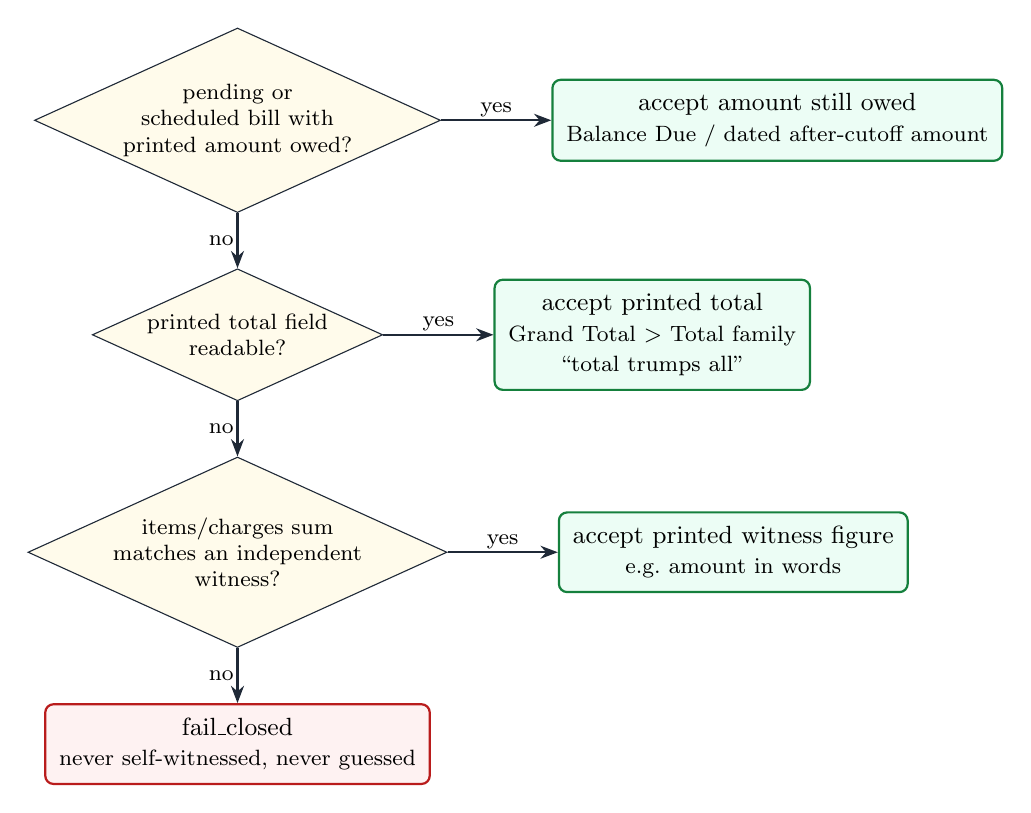
\begin{tikzpicture}[node distance=7mm and 10mm]
  \node[decision] (q1) {pending or\\scheduled bill with\\printed amount owed?};
  \node[good, right=14mm of q1] (a1) {accept amount still owed\\\footnotesize Balance Due / dated after-cutoff amount};
  \node[decision, below=of q1] (q2) {printed total field\\readable?};
  \node[good, right=14mm of q2] (a2) {accept printed total\\\footnotesize Grand Total $>$ Total family\\\footnotesize ``total trumps all''};
  \node[decision, below=of q2] (q3) {items/charges sum\\matches an independent\\witness?};
  \node[good, right=14mm of q3] (a3) {accept printed witness figure\\\footnotesize e.g.\ amount in words};
  \node[fail, below=of q3] (f) {fail\_closed\\\footnotesize never self-witnessed, never guessed};
  \draw[flow] (q1) -- node[lbl,above]{yes} (a1);
  \draw[flow] (q1) -- node[lbl,left]{no} (q2);
  \draw[flow] (q2) -- node[lbl,above]{yes} (a2);
  \draw[flow] (q2) -- node[lbl,left]{no} (q3);
  \draw[flow] (q3) -- node[lbl,above]{yes} (a3);
  \draw[flow] (q3) -- node[lbl,left]{no} (f);
\end{tikzpicture}
\caption{Figure selection. A detailed breakdown that does not sum never rejects a printed final amount (pages are often cropped). Cross-read and cutoff agreement checks remain in the gate.}
\end{figure}

Witness identities (\texttt{extract::witness::WitnessKind}): line-item sum, subtotal plus charges, subtotal plus tax,
gross minus deductions, paid plus balance, total minus paid, amount in words, repeated final label, after-cutoff amount
exceeding a witnessed before-cutoff amount, line-item sum witnessed by words or label, and printed-final-label-only.

\subsection{Results on the 16 images}
\begin{center}\small
\begin{tabular}{@{}lllrll@{}}
\toprule
Image & Event & Status & Accepted figure & Witness / reason & Scope\\\midrule
01 & net salary (IDR) & settled & 4{,}365{,}000 & gross $-$ deductions & sample\\
02 & outstanding rent balance & scheduled & 100{,}000 & total $-$ paid & sample\\
03 & bulk groceries & settled & 41{,}272 & repeated final label & sample\\
04 & delivered grocery order & settled & --- & fail\_closed: no final label (cropped) & sample\\
05 & outstanding telecom bill & pending & 822.05 & after-cutoff $>$ witnessed before-cutoff & sample\\
06 & grocery tax invoice & settled & 1{,}995 & item sum witnessed by words & eval\\
07 & restaurant tax invoice & settled & 8{,}528 & grand total & eval\\
08 & property maintenance & settled & 15{,}339 & line-item sum & eval\\
09 & water bill & settled & 723 & line-item sum & eval\\
10 & large grocery invoice (2 pages) & pending & 79{,}679.26 & amount in words & eval\\
11 & hospital bill & scheduled & 3{,}650 & repeated final label & eval\\
12 & taxi fare & settled & 33.50 USD & subtotal + tax & eval\\
13 & tote bag order & settled & 2{,}298 & repeated final label & eval\\
14 & pharmacy (handwritten) & settled & 4{,}543 & printed final label only & eval\\
15 & airline ticket & settled & 9{,}968 & line-item sum & eval\\
16 & EV charging & settled & 393.22 & amount in words & eval\\
\bottomrule
\end{tabular}
\end{center}
All accepted figures match the rulings recorded before the final run; 0 false accepts.

%=====================================================================
\section{Decision engine}
%=====================================================================

\begin{figure}[h]
\centering
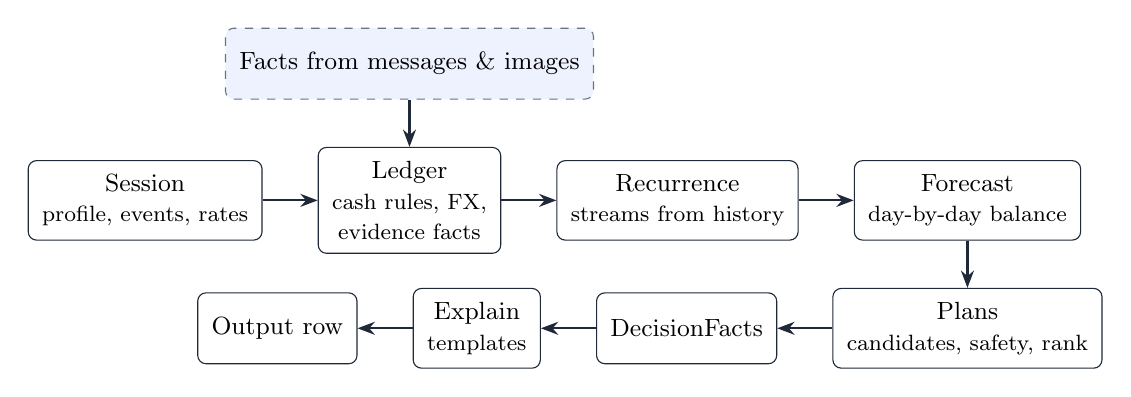
\begin{tikzpicture}[node distance=6mm and 7mm]
  \node[box] (sess) {Session\\\footnotesize profile, events, rates};
  \node[box, right=of sess] (led) {Ledger\\\footnotesize cash rules, FX,\\\footnotesize evidence facts};
  \node[box, right=of led] (rec) {Recurrence\\\footnotesize streams from history};
  \node[box, right=of rec] (fc) {Forecast\\\footnotesize day-by-day balance};
  \node[box, below=of fc] (pl) {Plans\\\footnotesize candidates, safety, rank};
  \node[box, left=of pl] (facts) {DecisionFacts};
  \node[box, left=of facts] (ex) {Explain\\\footnotesize templates};
  \node[box, left=of ex] (row) {Output row};
  \node[ext, above=of led] (ev) {Facts from messages \& images};
  \draw[flow] (sess) -- (led); \draw[flow] (led) -- (rec); \draw[flow] (rec) -- (fc); \draw[flow] (fc) -- (pl);
  \draw[flow] (pl) -- (facts); \draw[flow] (facts) -- (ex); \draw[flow] (ex) -- (row); \draw[flow] (ev) -- (led);
\end{tikzpicture}
\caption{Engine flow (\texttt{code/src/engine}). Pure functions of the inputs; no I/O.}
\end{figure}

\subsection{Ledger and cash rules}
\begin{itemize}[leftmargin=*,itemsep=1pt]
  \item \textbf{Settled} rows are already inside \texttt{current\_balance}. \textbf{Pending} debits are reserved; pending credits,
        bonuses, commissions, refunds, lottery proceeds and unrealized investment value are never counted until they settle.
  \item \textbf{Scheduled} rows and confirmed salary count on their settlement dates. Linked lifecycle chains are de-duplicated,
        because a link alone never decides cash treatment.
  \item \textbf{Foreign currency} converts with the \texttt{exchange\_rates.csv} row for the settlement date and stated direction.
        Converted amounts keep full precision; rounding happens only at output.
  \item \textbf{Evidence conflicts} resolve in the specified order: an explicit cancellation, settlement or amendment, then newer
        records from the same source, then a settled event, then the financially safer interpretation.
  \item \textbf{Percentage changes} (e.g.\ ``rent +12\%'') scale only recurring cycle rows, never a one-off scheduled balance.
\end{itemize}

\subsection{Forecast}
Let $b_t$ be the projected end-of-day balance on day $t$ of the horizon, $\ell_t$ the intraday low (debits applied before
that day's credits), $M$ the minimum balance to keep and $R$ the requested amount. With headroom $H_t=\ell_t-M$:
\[
  \text{safe} = \min\!\bigl(R,\ \max\bigl(0,\ \min_{t\ge 0} H_t\bigr)\bigr),\qquad
  E = \min\Bigl\{ d \;:\; \min\bigl(b_d,\ \min_{t>d}\ell_t\bigr) - M \ \ge R \Bigr\}.
\]
A payment on day $d$ lowers every later balance by the same amount, so suffix minima are computed once, making $E$
linear-time. Recurring variable spending is projected conservatively. Three rule toggles, selected by held-out A/B,
are on by default: fixed bills after salary credit on the same day, scheduled-row replacement by lifecycle or amount,
and a mid-step phase for long-interval variable streams.

\begin{figure}[h]
\centering
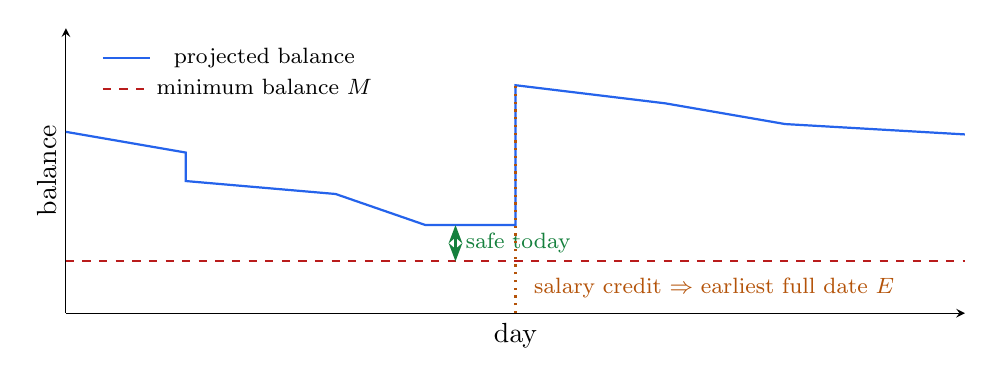
\begin{tikzpicture}
\begin{axis}[width=13cm,height=5.2cm,xlabel={day},ylabel={balance},ymin=0,ymax=11,xmin=0,xmax=30,
  axis lines=left,ticks=none,legend style={font=\footnotesize,draw=none},legend pos=north west]
  \addplot[thick,accent] coordinates {(0,7) (4,6.2) (4,5.1) (9,4.6) (12,3.4) (15,3.4) (15,8.8) (20,8.1) (24,7.3) (30,6.9)};
  \addlegendentry{projected balance}
  \addplot[thick,dashed,bad] coordinates {(0,2) (30,2)};
  \addlegendentry{minimum balance $M$}
  \draw[{Stealth}-{Stealth},ok,thick] (axis cs:13,2) -- node[right,font=\footnotesize]{safe today} (axis cs:13,3.4);
  \draw[dotted,thick,warn] (axis cs:15,0) -- (axis cs:15,8.8);
  \node[font=\footnotesize,warn,anchor=south west] at (axis cs:15.3,0.2) {salary credit $\Rightarrow$ earliest full date $E$};
\end{axis}
\end{tikzpicture}
\caption{Illustration. The safe amount is the minimum headroom over the horizon. $E$ is the first day from which the headroom never drops below $R$.}
\end{figure}

\subsection{Plans and ranking}
Candidates are a full payment today, each supplied installment option, a two-payment partial plan
(\texttt{amount\_safe\_to\_pay} today, the remainder on $E$, only if partial payment is allowed and $E\le$ desired
completion date), wait until $E$, and variants with up to three spending changes on non-protected, flexible events in
permitted categories. Every candidate is replayed day by day against the forecast. Candidates that would breach
$M$, violate user preferences or \texttt{max\_installment\_months}, or miss the deadline are dropped with a recorded
reason. Survivors rank lexicographically: completes by the deadline, avoids spending changes, minimizes total payment
cost, starts earlier, uses fewer payments.

\subsection{Explanations}
\texttt{DecisionFacts} records every number the recommendation rests on: balance, reserved pending debits, the forecast
trough and its drivers, accepted and unverified evidence, and plan rejections. \texttt{engine::explain} renders the
explanation from templates filled only from these facts, so the explanation cannot contradict the row and costs 0 tokens.

%=====================================================================
\section{Message evidence}
%=====================================================================
Messages are untrusted evidence. \texttt{extract::retrieval} selects the user's messages dated on or before the request
date. \texttt{extract::messages} converts known message families into typed records with a deterministic parser; the
final run made no language-model calls for messages. Every number a record claims must literally appear in the message
text (\texttt{extract::grounding}), and embedded instructions are never executed. Records become engine \texttt{Fact}s:
amendment, cancellation, settlement, confirmed income, expense amount change. Facts with no matching \texttt{Fact}
variant are dropped, never guessed.

%=====================================================================
\section{Verification and ship gate}
%=====================================================================

\begin{figure}[h]
\centering
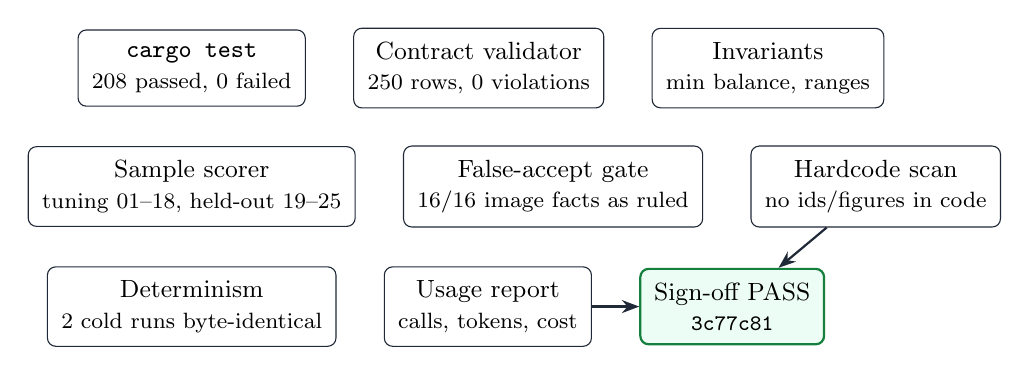
\begin{tikzpicture}[node distance=5mm and 6mm]
  \node[box] (t) {\texttt{cargo test}\\\footnotesize 208 passed, 0 failed};
  \node[box, right=of t] (c) {Contract validator\\\footnotesize 250 rows, 0 violations};
  \node[box, right=of c] (i) {Invariants\\\footnotesize min balance, ranges};
  \node[box, below=of t] (s) {Sample scorer\\\footnotesize tuning 01--18, held-out 19--25};
  \node[box, right=of s] (f) {False-accept gate\\\footnotesize 16/16 image facts as ruled};
  \node[box, right=of f] (h) {Hardcode scan\\\footnotesize no ids/figures in code};
  \node[box, below=of s] (d) {Determinism\\\footnotesize 2 cold runs byte-identical};
  \node[box, right=of d] (u) {Usage report\\\footnotesize calls, tokens, cost};
  \node[good, right=of u] (ok) {Sign-off PASS\\\footnotesize \texttt{3c77c81}};
  \draw[flow] (h) -- (ok); \draw[flow] (u) -- (ok);
\end{tikzpicture}
\caption{The ship gate (\texttt{evaluation::signoff}) requires every check to pass on one commit.}
\end{figure}

\noindent The sample scorer keeps held-out labels out of the tuning loop: held-out rows report pass counts only. Every rule
change shipped as a separate commit with a moved-row check against the previous output.

%=====================================================================
\section{Requirements traceability}
%=====================================================================
\begin{longtable}{p{5.2cm} p{6.4cm} p{3.4cm}}
\toprule
\textbf{Requirement (AGENTS.md / problem)} & \textbf{Implementation} & \textbf{Evidence}\\\midrule
\endhead
One row per request, exact header & \texttt{main.rs} writer + \texttt{evaluation::contract} & 250/250, 0 violations\\
\texttt{amount\_safe\_to\_pay} in $[0,R]$ & forecast clamp & validator\\
\texttt{affordable\_now} $\Rightarrow$ $E$ = request date & forecast $E$ & validator\\
Partial plan: exactly two payments summing to $R$ & \texttt{plans} candidate rules & validator\\
Installments follow a supplied option & \texttt{plans} over \texttt{request\_payment\_options.csv} & validator\\
$\le$3 spending changes, permitted events only & \texttt{plans} + profile categories & validator\\
Never below minimum balance & per-day replay & invariants\\
Reserve pending debits; ignore unsettled credits & \texttt{ledger} cash rules & scenario tests\\
Confirmed salary on settlement date & \texttt{ledger}, \texttt{recurrence} & scenario tests\\
FX by settlement-date row & \texttt{ledger} & scenario tests\\
Conflict resolution order & \texttt{ledger::apply\_evidence} & scenario tests\\
Messages and images untrusted & grounding + witness gate & false-accept gate\\
Deterministic & fixed-point money, temp 0, config-hashed cache & byte-identical runs\\
Secrets from environment only & \texttt{.env} loader; zip excludes \texttt{.env} & zip scan\\
No organizer files or hardcoded labels & \texttt{evaluation::hardcode\_scan} & clean\\
Usage report & \texttt{evaluation/usage\_report.md} & present\\
\bottomrule
\end{longtable}

%=====================================================================
\section{Operations}
%=====================================================================
\begin{lstlisting}
# 1) OCR server (any NVIDIA host; POC used a RunPod H100)
docker run --rm --gpus all --network host --ipc host \
  vllm/vllm-openai:unlimited-ocr-cu129 baidu/Unlimited-OCR --trust-remote-code \
  --logits_processors vllm.model_executor.models.unlimited_ocr:NGramPerReqLogitsProcessor \
  --no-enable-prefix-caching --mm-processor-cache-gb 0 --host 0.0.0.0 --port 8000

# 2) Environment (code/.env, never committed)
OCR_BASE_URL=http://<host>:8000/v1

# 3) Run (from code/)
CARGO_TARGET_DIR=target cargo run --release -- --cold          # submission run
CARGO_TARGET_DIR=target cargo run --release -- --requests ../dataset/sample_requests.csv --out /tmp/s.csv
CARGO_TARGET_DIR=target cargo test
\end{lstlisting}
Ingestion is cache-first: pages already in \texttt{code/store/ocr/} under the same config hash are reused, and only
missing pages call the endpoint. \texttt{-{}-cold} wipes the processed store so every OCR call in the usage report is real.
\texttt{HF\_TOKEN} is not required for the default configuration.

%=====================================================================
\section{Known limitations and next steps}
%=====================================================================
\begin{itemize}[leftmargin=*,itemsep=2pt]
  \item \textbf{Cropped documents.} Image 04 has no printed total. It fails closed by design and its settled amount stays unknown.
  \item \textbf{Serving-stack variance.} vLLM and the transformers reference implementation differ on a few table cells (image 06's
        total cell, image 14's split total). Both are deterministic, and the witness rules recover the figures.
        A resolver model that only points at printed rows (Rust re-verifies) is a planned extension.
  \item \textbf{Handwriting.} Line items on image 14 are misread; only its printed total is used.
  \item \textbf{Unauthenticated POC endpoint.} Production needs an API key (\texttt{OCR\_API\_KEY}) and private networking.
  \item \textbf{Small labelled sample.} 25 sample requests (7 held out) limit how precisely rule toggles can be validated.
  \item \textbf{Legacy readers.} The Hugging Face VLM and Anthropic paths remain compiled but switched off; they could be removed to shrink the attack and maintenance surface.
\end{itemize}

\end{document}
